% A LaTeX template for MSc Thesis submissions to 
% Politecnico di Milano (PoliMi) - School of Industrial and Information Engineering
%
% S. Bonetti, A. Gruttadauria, G. Mescolini, A. Zingaro
% e-mail: template-tesi-ingind@polimi.it
%
% Last Revision: October 2021
%
% Copyright 2021 Politecnico di Milano, Italy. NC-BY

\documentclass{Configuration_Files/PoliMi3i_thesis}

%------------------------------------------------------------------------------
%	REQUIRED PACKAGES AND  CONFIGURATIONS
%------------------------------------------------------------------------------

% CONFIGURATIONS
\usepackage{parskip} % For paragraph layout
\usepackage{setspace} % For using single or double spacing
\usepackage{emptypage} % To insert empty pages
\usepackage{multicol} % To write in multiple columns (executive summary)
\setlength\columnsep{15pt} % Column separation in executive summary
\setlength\parindent{0pt} % Indentation
\raggedbottom  

% PACKAGES FOR TITLES
\usepackage{titlesec}
% \titlespacing{\section}{left spacing}{before spacing}{after spacing}
\titlespacing{\section}{0pt}{3.3ex}{2ex}
\titlespacing{\subsection}{0pt}{3.3ex}{1.65ex}
\titlespacing{\subsubsection}{0pt}{3.3ex}{1ex}
\usepackage{color}

% PACKAGES FOR LANGUAGE AND FONT
\usepackage[english]{babel} % The document is in English  
\usepackage[utf8]{inputenc} % UTF8 encoding
\usepackage[T1]{fontenc} % Font encoding
\usepackage[11pt]{moresize} % Big fonts

% PACKAGES FOR IMAGES
\usepackage{graphicx}
\usepackage{transparent} % Enables transparent images
\usepackage{eso-pic} % For the background picture on the title page
\usepackage{subfig} % Numbered and caption subfigures using \subfloat.
\usepackage{tikz} % A package for high-quality hand-made figures.
\usetikzlibrary{}
\graphicspath{{./Images/}} % Directory of the images
\usepackage{caption} % Coloured captions
\usepackage{xcolor} % Coloured captions
\usepackage{amsthm,thmtools,xcolor} % Coloured "Theorem"
\usepackage{float}

% STANDARD MATH PACKAGES
\usepackage{amsmath}
\usepackage{amsthm}
\usepackage{amssymb}
\usepackage{amsfonts}
\usepackage{bm}
\usepackage[overload]{empheq} % For braced-style systems of equations.
\usepackage{fix-cm} % To override original LaTeX restrictions on sizes

% PACKAGES FOR TABLES
\usepackage{tabularx}
\usepackage{longtable} % Tables that can span several pages
\usepackage{colortbl}

% PACKAGES FOR ALGORITHMS (PSEUDO-CODE)
\usepackage{algorithm}
\usepackage{algorithmic}

% PACKAGES FOR REFERENCES & BIBLIOGRAPHY
\usepackage[colorlinks=true,linkcolor=black,anchorcolor=black,citecolor=black,filecolor=black,menucolor=black,runcolor=black,urlcolor=black]{hyperref} % Adds clickable links at references
\usepackage{cleveref}
\usepackage[square, numbers, sort&compress]{natbib} % Square brackets, citing references with numbers, citations sorted by appearance in the text and compressed
%\bibliographystyle{abbrvnat} % You may use a different style adapted to your field
\bibliographystyle{unsrtnat} % This is used to sort references by appearance in the text

% OTHER PACKAGES
\usepackage{pdfpages} % To include a pdf file
\usepackage{afterpage}
\usepackage{lipsum} % DUMMY PACKAGE
\usepackage{fancyhdr} % For the headers
\usepackage{array}
\newcolumntype{P}[1]{>{\raggedright\arraybackslash}p{#1}}
\fancyhf{}

% Input of configuration file. Do not change config.tex file unless you really know what you are doing. 
% Define blue color typical of polimi
\definecolor{bluepoli}{cmyk}{0.4,0.1,0,0.4}

% Custom theorem environments
\declaretheoremstyle[
  headfont=\color{bluepoli}\normalfont\bfseries,
  bodyfont=\color{black}\normalfont\itshape,
]{colored}

% Set-up caption colors
\captionsetup[figure]{labelfont={color=bluepoli}} % Set colour of the captions
\captionsetup[table]{labelfont={color=bluepoli}} % Set colour of the captions
\captionsetup[algorithm]{labelfont={color=bluepoli}} % Set colour of the captions

\theoremstyle{colored}
\newtheorem{theorem}{Theorem}[chapter]
\newtheorem{proposition}{Proposition}[chapter]

% Enhances the features of the standard "table" and "tabular" environments.
\newcommand\T{\rule{0pt}{2.6ex}}
\newcommand\B{\rule[-1.2ex]{0pt}{0pt}}

% Pseudo-code algorithm descriptions.
\newcounter{algsubstate}
\renewcommand{\thealgsubstate}{\alph{algsubstate}}
\newenvironment{algsubstates}
  {\setcounter{algsubstate}{0}%
   \renewcommand{\STATE}{%
     \stepcounter{algsubstate}%
     \Statex {\small\thealgsubstate:}\space}}
  {}

% New font size
\newcommand\numfontsize{\@setfontsize\Huge{200}{60}}

% Title format: chapter
\titleformat{\chapter}[hang]{
\fontsize{50}{20}\selectfont\bfseries\filright}{\textcolor{bluepoli} \thechapter\hsp\hspace{2mm}\textcolor{bluepoli}{|   }\hsp}{0pt}{\huge\bfseries \textcolor{bluepoli}
}

% Title format: section
\titleformat{\section}
{\color{bluepoli}\normalfont\Large\bfseries}
{\color{bluepoli}\thesection.}{1em}{}

% Title format: subsection
\titleformat{\subsection}
{\color{bluepoli}\normalfont\large\bfseries}
{\color{bluepoli}\thesubsection.}{1em}{}

% Title format: subsubsection
\titleformat{\subsubsection}
{\color{bluepoli}\normalfont\large\bfseries}
{\color{bluepoli}\thesubsubsection.}{1em}{}

% Shortening for setting no horizontal-spacing
\newcommand{\hsp}{\hspace{0pt}}

\makeatletter
% Renewcommand: cleardoublepage including the background pic
\renewcommand*\cleardoublepage{%
  \clearpage\if@twoside\ifodd\c@page\else
  \null
  \AddToShipoutPicture*{\BackgroundPic}
  \thispagestyle{empty}%
  \newpage
  \if@twocolumn\hbox{}\newpage\fi\fi\fi}
\makeatother

%For correctly numbering algorithms
\numberwithin{algorithm}{chapter}

%----------------------------------------------------------------------------
%	NEW COMMANDS DEFINED
%----------------------------------------------------------------------------

% EXAMPLES OF NEW COMMANDS
\newcommand{\bea}{\begin{eqnarray}} % Shortcut for equation arrays
\newcommand{\eea}{\end{eqnarray}}
\newcommand{\e}[1]{\times 10^{#1}}  % Powers of 10 notation

%----------------------------------------------------------------------------
%	ADD YOUR PACKAGES (be careful of package interaction)
%----------------------------------------------------------------------------

%----------------------------------------------------------------------------
%	ADD YOUR DEFINITIONS AND COMMANDS (be careful of existing commands)
%----------------------------------------------------------------------------

%----------------------------------------------------------------------------
%	BEGIN OF YOUR DOCUMENT
%----------------------------------------------------------------------------

\begin{document}

\fancypagestyle{plain}{%
\fancyhf{} % Clear all header and footer fields
\fancyhead[RO,RE]{\thepage} %RO=right odd, RE=right even
\renewcommand{\headrulewidth}{0pt}
\renewcommand{\footrulewidth}{0pt}}

%----------------------------------------------------------------------------
%	TITLE PAGE
%----------------------------------------------------------------------------

\pagestyle{empty} % No page numbers
\frontmatter % Use roman page numbering style (i, ii, iii, iv...) for the preamble pages

\puttitle{
	title=Title, % Title of the thesis
	name=Matteo Venturelli, % Author Name and Surname
	course=Engineering Physics - Ingegneria Fisica, % Study Programme (in Italian)
	ID  = 995709,  % Student ID number (numero di matricola)
	advisor= Prof. Giacomo Claudio Ghiringhelli, % Supervisor name
	coadvisor={Matilda Fransson, Ludovic Broche}, % Co-Supervisor name, remove this line if there is none
	academicyear={2023-24},  % Academic Year
} % These info will be put into your Title page 

%----------------------------------------------------------------------------
%	PREAMBLE PAGES: ABSTRACT (inglese e italiano), EXECUTIVE SUMMARY
%----------------------------------------------------------------------------
\startpreamble
\setcounter{page}{1} % Set page counter to 1

% ABSTRACT IN ENGLISH
\chapter*{Abstract} 
Here goes the Abstract in English of your thesis followed by a list of keywords.
The Abstract is a concise summary of the content of the thesis (single page of text)
and a guide to the most important contributions included in your thesis.
The Abstract is the very last thing you write.
It should be a self-contained text and should be clear to someone who hasn't (yet) read the whole manuscript.
The Abstract should contain the answers to the main scientific questions that have been addressed in your thesis.
It needs to summarize the adopted motivations and the adopted methodological approach as well as the findings of your work and their relevance and impact.
The Abstract is the part appearing in the record of your thesis inside POLITesi,
the Digital Archive of PhD and Master Theses (Laurea Magistrale) of Politecnico di Milano.
The Abstract will be followed by a list of four to six keywords.
Keywords are a tool to help indexers and search engines to find relevant documents.
To be relevant and effective, keywords must be chosen carefully.
They should represent the content of your work and be specific to your field or sub-field.
Keywords may be a single word or two to four words. 
\\
\\
\textbf{Keywords:} here, the keywords, of your thesis % Keywords

% ABSTRACT IN ITALIAN
\chapter*{Abstract in lingua italiana}
Qui va l'Abstract in lingua italiana della tesi seguito dalla lista di parole chiave.
\\
\\
\textbf{Parole chiave:} qui, vanno, le parole chiave, della tesi % Keywords (italian)

%----------------------------------------------------------------------------
%	LIST OF CONTENTS/FIGURES/TABLES/SYMBOLS
%----------------------------------------------------------------------------

% TABLE OF CONTENTS
\thispagestyle{empty}
\tableofcontents % Table of contents 
\thispagestyle{empty}
\cleardoublepage

%-------------------------------------------------------------------------
%	THESIS MAIN TEXT
%-------------------------------------------------------------------------
% In the main text of your thesis you can write the chapters in two different ways:
%
%(1) As presented in this template you can write:
%    \chapter{Title of the chapter}
%    *body of the chapter*
%
%(2) You can write your chapter in a separated .tex file and then include it in the main file with the following command:
%    \chapter{Title of the chapter}
%    \input{chapter_file.tex}
%
% Especially for long thesis, we recommend you the second option.

\addtocontents{toc}{\vspace{2em}} % Add a gap in the Contents, for aesthetics
\mainmatter % Begin numeric (1,2,3...) page numbering

% --------------------------------------------------------------------------
% NUMBERED CHAPTERS % Regular chapters following
% --------------------------------------------------------------------------
\chapter*{Introduction}
\label{ch:introduction}%
Here goes the introduction of your thesis.

\chapter{Lithium-ion batteries}
\label{ch:li-ion}%
% Here goes the introduction to Li-ion Batteries (LIBs). This includes the discussion of the topics mentioned in the introduction and graphs about co2 emission and the role of transportation sector in it.

The Earth stands at a critical juncture in its history, where the consequences of human activity on the environment have reached a crossroads of global significance. Climate change, driven primarily by the relentless emission of greenhouse gases, has manifested itself in increasingly severe weather patterns, rising sea levels, and ecological disruptions. The urgency of the situation cannot be overstated, as nations grapple with the complex challenge of reducing carbon dioxide (CO$_2$) emissions to mitigate the impending climate crisis. 

The transportation sector emerges as a critical contributor to the climate change predicament. As societies evolve and the global population continues to grow, the demand for transportation, particularly in the form of automobiles and other fossil-fuel-reliant means, has risen dramatically. These modes of transportation are notorious for their carbon emissions, releasing vast amounts of CO2 into the atmosphere. Consequently, the transportation sector plays a pivotal role in the collective effort to address the climate crisis. 

The dire need for sustainable energy solutions has never been more evident. While various sectors of the economy are challenged to reduce their carbon footprint, the transportation sector presents a unique dilemma. As people's mobility requirements persist, innovative solutions are crucial to decouple the connection between personal mobility and CO2 emissions. Electric vehicles (EVs) have emerged as a promising alternative to traditional internal combustion engine vehicles. They offer the potential to revolutionize the way we commute, significantly diminishing the transportation sector's contribution to carbon emissions. 

At the heart of the electric vehicle industry's transformation lies lithium-ion batteries. These energy storage devices have rapidly gained prominence as the primary means of powering EVs. The suitability of lithium-ion batteries for this role is driven by their impressive energy density, rechargeability, and relatively low environmental impact compared to conventional fossil fuels. As we explore the potential of lithium-ion batteries, it becomes evident that their development and adoption may hold the key to mitigating the environmental impact of the transportation sector. 

Lithium-ion batteries offer several key advantages that make them a compelling solution to the challenge of reducing CO$_2$ emissions in the transportation sector. Their high energy density allows electric vehicles to cover significant distances on a single charge, meeting the practical demands of modern commuting. Their rechargeability ensures that these batteries can be reused, reducing waste and minimizing their environmental footprint. Furthermore, the manufacturing and disposal of lithium-ion batteries have a comparatively lower impact on the environment when compared to the extraction and combustion of fossil fuels.

\section{Overview}
\label{sec:overview}

\subsection{Anode}
\label{sec:anode}

\subsection{Cathode}
\label{sec:cathode}

\subsection{Electrolyte}
\label{sec:electrolyte}

\subsection{Separator}
\label{sec:separator}

\subsection{Current Collectors}
\label{sec:current-collectors}

\subsection{Cell Geometries and Designs}
\label{sec:cell-geometries-designs}

\section{Safety and Degradation}
\label{sec:safety-degradation}


\chapter{Battery Failure}
\label{ch:failure}%
The increasing interest in lithium-ion batteries stems from their potential to offer efficient energy storage and contribute to environmental sustainability. Not only are LIBs widely employed in portable electronics like computers and cell phones, but they have also become integral to the power systems of electric and hybrid vehicles. The increasing popularity of LIBs in these applications can be attributed to their outstanding performance and high energy density \cite{kang2020binder}. Moreover, LIBs dominate the battery market for portable electronics, owing to inherent advantages such as high specific capacity and voltage, absence of memory effect, excellent cycling performance, minimal self-discharge, and a wide temperature range of operation \cite{zubi2018lithium}.

\vspace{5mm}

\begin{table}[ht]
    \centering
        \begin{footnotesize}
            \begin{tabular}{|p{7mm} p{22mm} p{113mm}|}
                \hline
                \rowcolor{bluepoli!40}
                \textbf{No.} & \textbf{Date} & \textbf{Accidents Replay}\T\B \\
                \hline \hline
                1 & Mar 2010 & Two iPod Nano music players overheated and caught fire, Japan\T\B\\
                2 & Apr 2010 & Acer recalled 2700 laptop batteries, as Dell, Apple, Toshiba, Lenovo and Sony did in 2006\T\B\\
                3 & Apr 2011 & EV taxi caught fire, Hangzhou, China\T\B\\
                4 & Jan-Dec 2013 & Three fire accidents of Boeing 747, happened in Boston America, Takamatsu, Tokyo Japan, respectively\T\B\\
                5 & Oct-Nov 2013 & 6 Tesla Model S EV cars caught fire\T\B\\
                6 & Apr 2015 & EV bus caught fire during charge, Shenzhen, China\T\B\\
                7 & May 2016 & The storage room of the LIB caught explosion, Jiangsu, China\T\B\\
                8 & Aug 2016 & Samsung Note 7 smart phone explosion\T\B\\
                9 & May 2017 & Panasonic announced to recall over 270 thousand LIBs\T\B\\
                10 & Oct 2017 & EV car caught fire, Austria\T\B\\
                11 & Jan 2018 & Tesla Model S EV car self-ignited, China\T\B\\
                12 & Jul 2018 & 4 MW/12 MWh energy storage system (ESS) caught fire and explosion, Korea\T\B\\
                13 & Jul 2018 & Electric scooter caught fire and explosion during charging, China\T\B\\
                \hline
                \end{tabular}
                \\[10pt]
                \caption[Lithium-ion battery accidents]{Lithium-ion battery fire and explosion accidents in the past few years. Source: Wang (2019) \cite{wang2019review}.}
                \label{table:accidents}
        \end{footnotesize}
\end{table}


Despite these merits, the broader expansion of the LIB market, especially in electric vehicles, faces significant challenges due to safety concerns \cite{love2018innovating,schipper2016recent,feng2018thermal}. Recent years have witnessed numerous recalls of LIBs, prompted by incidents of explosions and fires (Table \ref{table:accidents}), leading to substantial economic repercussions in related market sectors and tarnishing the reputation of LIBs \cite{chen2021review,balakrishnan2006safety}. As a result, there is a growing emphasis on addressing LIB safety issues, with the development of numerous safety strategies aimed at mitigating the risks associated with these batteries.

\section{Safety Standards}
\label{sec:safety-standards}

Safety standards and corresponding assessments have been established to analyze battery performance and key factors, aligning with the necessary safety requisites. The stringent and rigorous battery safety tests are designed to minimize the likelihood of safety issues in routine working conditions and ensure that batteries available on the market are of sufficient quality for intended purposes. Thanks to these measures, contemporary LIBs exhibit a significantly enhanced safety profile compared to their predecessors. Nonetheless, ongoing advancements are imperative to further improve battery safety standards \cite{chen2021review}.

Hence, various international safety organizations regulate battery safety, and governments of different countries have formulated safety standards in accordance with national requirements and conditions and have gradually improved the safety standards of lithium-ion batteries. Academics and industrial groups have also carried out extensive research on battery safety.

Most countries and international organizations have developed LIB safety oriented standards, which include:
\begin{enumerate}
    \item Chinese standard GB/T 31485 \cite{};
    \item Society of Automotive Engineers (SAE) standard 2464 \cite{};
    \item International Electrotechnical Commission (IEC) standard IEC62133 Edition 2.0 \cite{};
    \item United Nations (UN) standard UN38.3 \cite{};
    \item Japanese Industrial Standard (JIS) C8714 \cite{};
    \item Underwriters Laboratories (UL) standard UL2580 Edition 2.0 \cite{};
    \item International Standardization Organization (ISO) standard ISO 16750-2 \cite{}.
\end{enumerate}

Since the various safety test standars apply different methodologies, a summary of some test requirements and comparisons of five test items are presented in Table \ref{table:standards}.

\begin{table}[ht]
    \centering
        \begin{scriptsize}
            \begin{tabular}{|P{20mm} P{29mm} P{29mm} P{29mm} P{29mm}|}
                \hline
                \rowcolor{bluepoli!40}
                 & \textbf{GB/T31485} & \textbf{IEC62133} & \textbf{UL2580} & \textbf{SAE J2464}\T\B \\
                \hline \hline
                \textbf{Heating} & Heating at 5 $^\circ$C/min from 25 $^\circ$C to 130 $^\circ$C, hold for 30 mins \vspace{3mm}& 130 $^\circ$C, 10 mins & 150 $\pm$ 2 $^\circ$C, 60 mins & Max. stable temperature\T\B\\

                \textbf{Short-circuit} & Short circuit for 10 mins, $R\leq$ 5m$\Omega$ & 80$\pm$20m$\Omega$ & Short with $R\leq$ 5m$\Omega$ until explosion, fire or no temp change & $R\leq$ 5m$\Omega$ for hard short; $R\geq$ 5m$\Omega$ for soft short\vspace{3mm}\T\B\\

                \textbf{Overcharge} & 100\% SOC Overcharge to 1.5 $V_{max}$ or charge for 1 hour at 1C \vspace{3mm}& Overcharge to 250\% SOC at 1C & Overcharge to 200\% SOC at 1C & Overcharge to 200\% SOC at 1C\T\B\\

                \textbf{Over-discharge} & Over-discharge the 100\% SOC cell at 1C for 1.5 hours \vspace{3mm}& Over-discharge the 0\% SOC cell at 1C for 90 mins & Over-discharge the 0\% SOC cell at 1C for 90 mins & Over-discharge the cell to -100\% SOC\T\B\\

                \textbf{Nail penetration} & Penetration rate 25 mm/s, $\varphi$ 5$\sim$8mm, 100\% depth & / & 80 mm/s, $\varphi$ 3mm, 100\% depth & 80 mm/s, $\varphi$ 3mm, 100\% depth\T\B\\
                \hline
                \end{tabular}
                \\[10pt]
                \caption[Testing standards coparison]{Testing standards comparison of selected items. $\varphi$ represents the nail diameter. Source: Chen (2021) \cite{chen2021review}.}
                \label{table:standards}
        \end{scriptsize}
\end{table}



\subsection{Safety Tests}
\label{sec:safety-tests}
Analysis of the presence of various LIB defects and shortcomings can help to define specific LIB safety issues or hazards. Extensive testing uncovers these issues to assist efforts to ensure that future generations of batteries are safer and more reliable. In a safety test possible trigger modes are simplified so batteries thermal runaway characteristics are measurable in the laboratory. Laboratory environment test conditions must generally be more stringent than "real-world" conditions to ensure safety during actual use. For example, batteries being tested have to be maintained at a 100\% state of charge (SOC). The three principles of operability, repeatability and reproducibility should be met in the process of formulating a safety standard. 

Here follows a brief description of the main safety tests used to examine key LIB properties:

\begin{itemize}
    \item[--] \textbf{Overcharge tests} are intended to assess overcharge/over-discharge processes that occur in a cell when the charge and discharge process is out of control. According to the IEC standard test, the cell is first discharged to 3.0 V, and then is charged under 10 V. If the battery does not combust or explode during or after the test it is considered safe, its materials (electrolyte, active electrode materials, separators etc.) are regarded as having adequate properties, and the structural design is deemed satisfactory. The safety performance under overcharge is closely related to the charge rate, so overcharging is performed at different rates to establish at which extreme rate and voltage failure occurs;
    \item[--] \textbf{Heating tests} assess the thermal runaway caused by a battery being heated due to local overheating, and the subsequent thermal runaway expansion. Heating is used to analyze LIBs' thermal stability and heat distribution to ensure they have sufficiently efficient heat management and capability to forecast potential hazards. The results are then used to assess how thermal abuse consequences can be alleviated. Specifically, data obtained from hot box experiments are used to simulate their thermal characteristics, and distributions of internal and external temperatures, then assess possible improvements in their design, materials, cooling systems, etc.;
    \item \textbf{External short circuit tests} assess the short circuiting that is caused by external electrical connections of battery poles under abnormal conditions. According to the GB31485-2015 procedure, the battery is kept at 25 $\pm$ 2 $^\circ$C in a fully charged state for 30 minutes, then the cathode and anode terminals are connected with a wire, and the external resistance is kept at 5 m$\Omega$. During this test, the temperature and voltage are monitored simultaneously, throughout the entire test. The test is considered successful if the cell does not explode or combust;
    \item \textbf{Internal short circuit (ISC) tests} assess the short circuiting that is caused by internal electrical connections of battery poles under abnormal conditions. Several methods are used to initiate an internal short circuits, including nail penetration, heavy impact, crush and forced ISC. Nail penetration tests are the most common type of ISC tests, and they are designed to simulate internal battery short circuits that may occur when a battery's internal membrane is penetrated by impurities. According to GB/ T 31485, a fully-charged battery should be penetrated with a high temperature-resistant steel spike of $\varphi$ 5$\sim$8 mm in a direction perpendicular to the polar plate at a speed of 25 $\pm$ 5 mm/s. The penetration position should also be close to the geometric center of the penetrated surface, with the steel spike retained inside the battery. The test is considered successful if the cell does not explode or combust.
\end{itemize}

\subsection{Hazard level}
\label{sec:hazard-level}
In evaluations of batteries' safety condition based on results of the above abuse tests, the EUCAR Hazard Levels and the associated criteria that are widely applied. Typically, hazard levels of Electrical Energy Storage System (EESS) devices according to their responses to abuse conditions are assigned by EUCAR and presented in Table \ref{table:eucar}. Manufacturers and integrators may find it helpful and useful to take these levels into consideration when evaluating a given EESS design's abuse response.

\begin{table}[ht]
    \centering
        \begin{footnotesize}
            \begin{tabular}{|p{13mm} p{28mm} p{102mm}|}
                \hline
                \rowcolor{bluepoli!40}
                \textbf{Hazard Level} & \textbf{Description} & \textbf{Classification Criteria \& Effect}\T\B \\
                \hline \hline
                0 & No effect & No effect. No loss of functionality.\T\B\\
                \hline
                1 & Passive protection activated & No defect; no leakage; no venting, fire or flame; no rupture; no explosion; no exotermic reaction or thermal runaway. Cell reversibly damaged. Repair of protection device needed.\T\B\\
                \hline
                2 & Defect/Damage & No leakage; no venting, fire or flame; no rupture; no explosion; no exotermic reaction or thermal runaway. Cell irreversibly damaged. Repair needed.\T\B\\
                \hline
                3 & Leakage & No venting, fire or flame; no rupture; no explosion.\\
                & ($\Delta$ mass $<$ 50\%) & Weight loss $<$ 50\% of electrolyte weight (electrolyte = solvent + salt).\T\B\\
                \hline
                4 & Venting & No fire or flame; no rupture; no explosion.\\
                & ($\Delta$ mass $\geq$ 50\%) & Weight loss $\geq$ 50\% of electrolyte weight (electrolyte = solvent + salt).\T\B\\
                \hline
                5 & Fire or Flame & No rupture; no explosion (i.e. no flying parts).\T\B\\
                \hline
                6 & Rupture & No explosion, but flying parts of the active mass.\T\B\\
                \hline
                7 & Explosion & Explosion (i.e. disintegration of the cell).\T\B\\
                \hline
                \end{tabular}
                \\[10pt]
                \caption[EUCAR hazard levels]{EUCAR hazard levels and associated criteria. Source: EUCAR (2019) \cite{eucar2019}.}
                \label{table:eucar}
        \end{footnotesize}
\end{table}

\section{Thermal Runaway}
\label{sec:thermal-runaway}

\begin{figure}[ht]
    \centering
    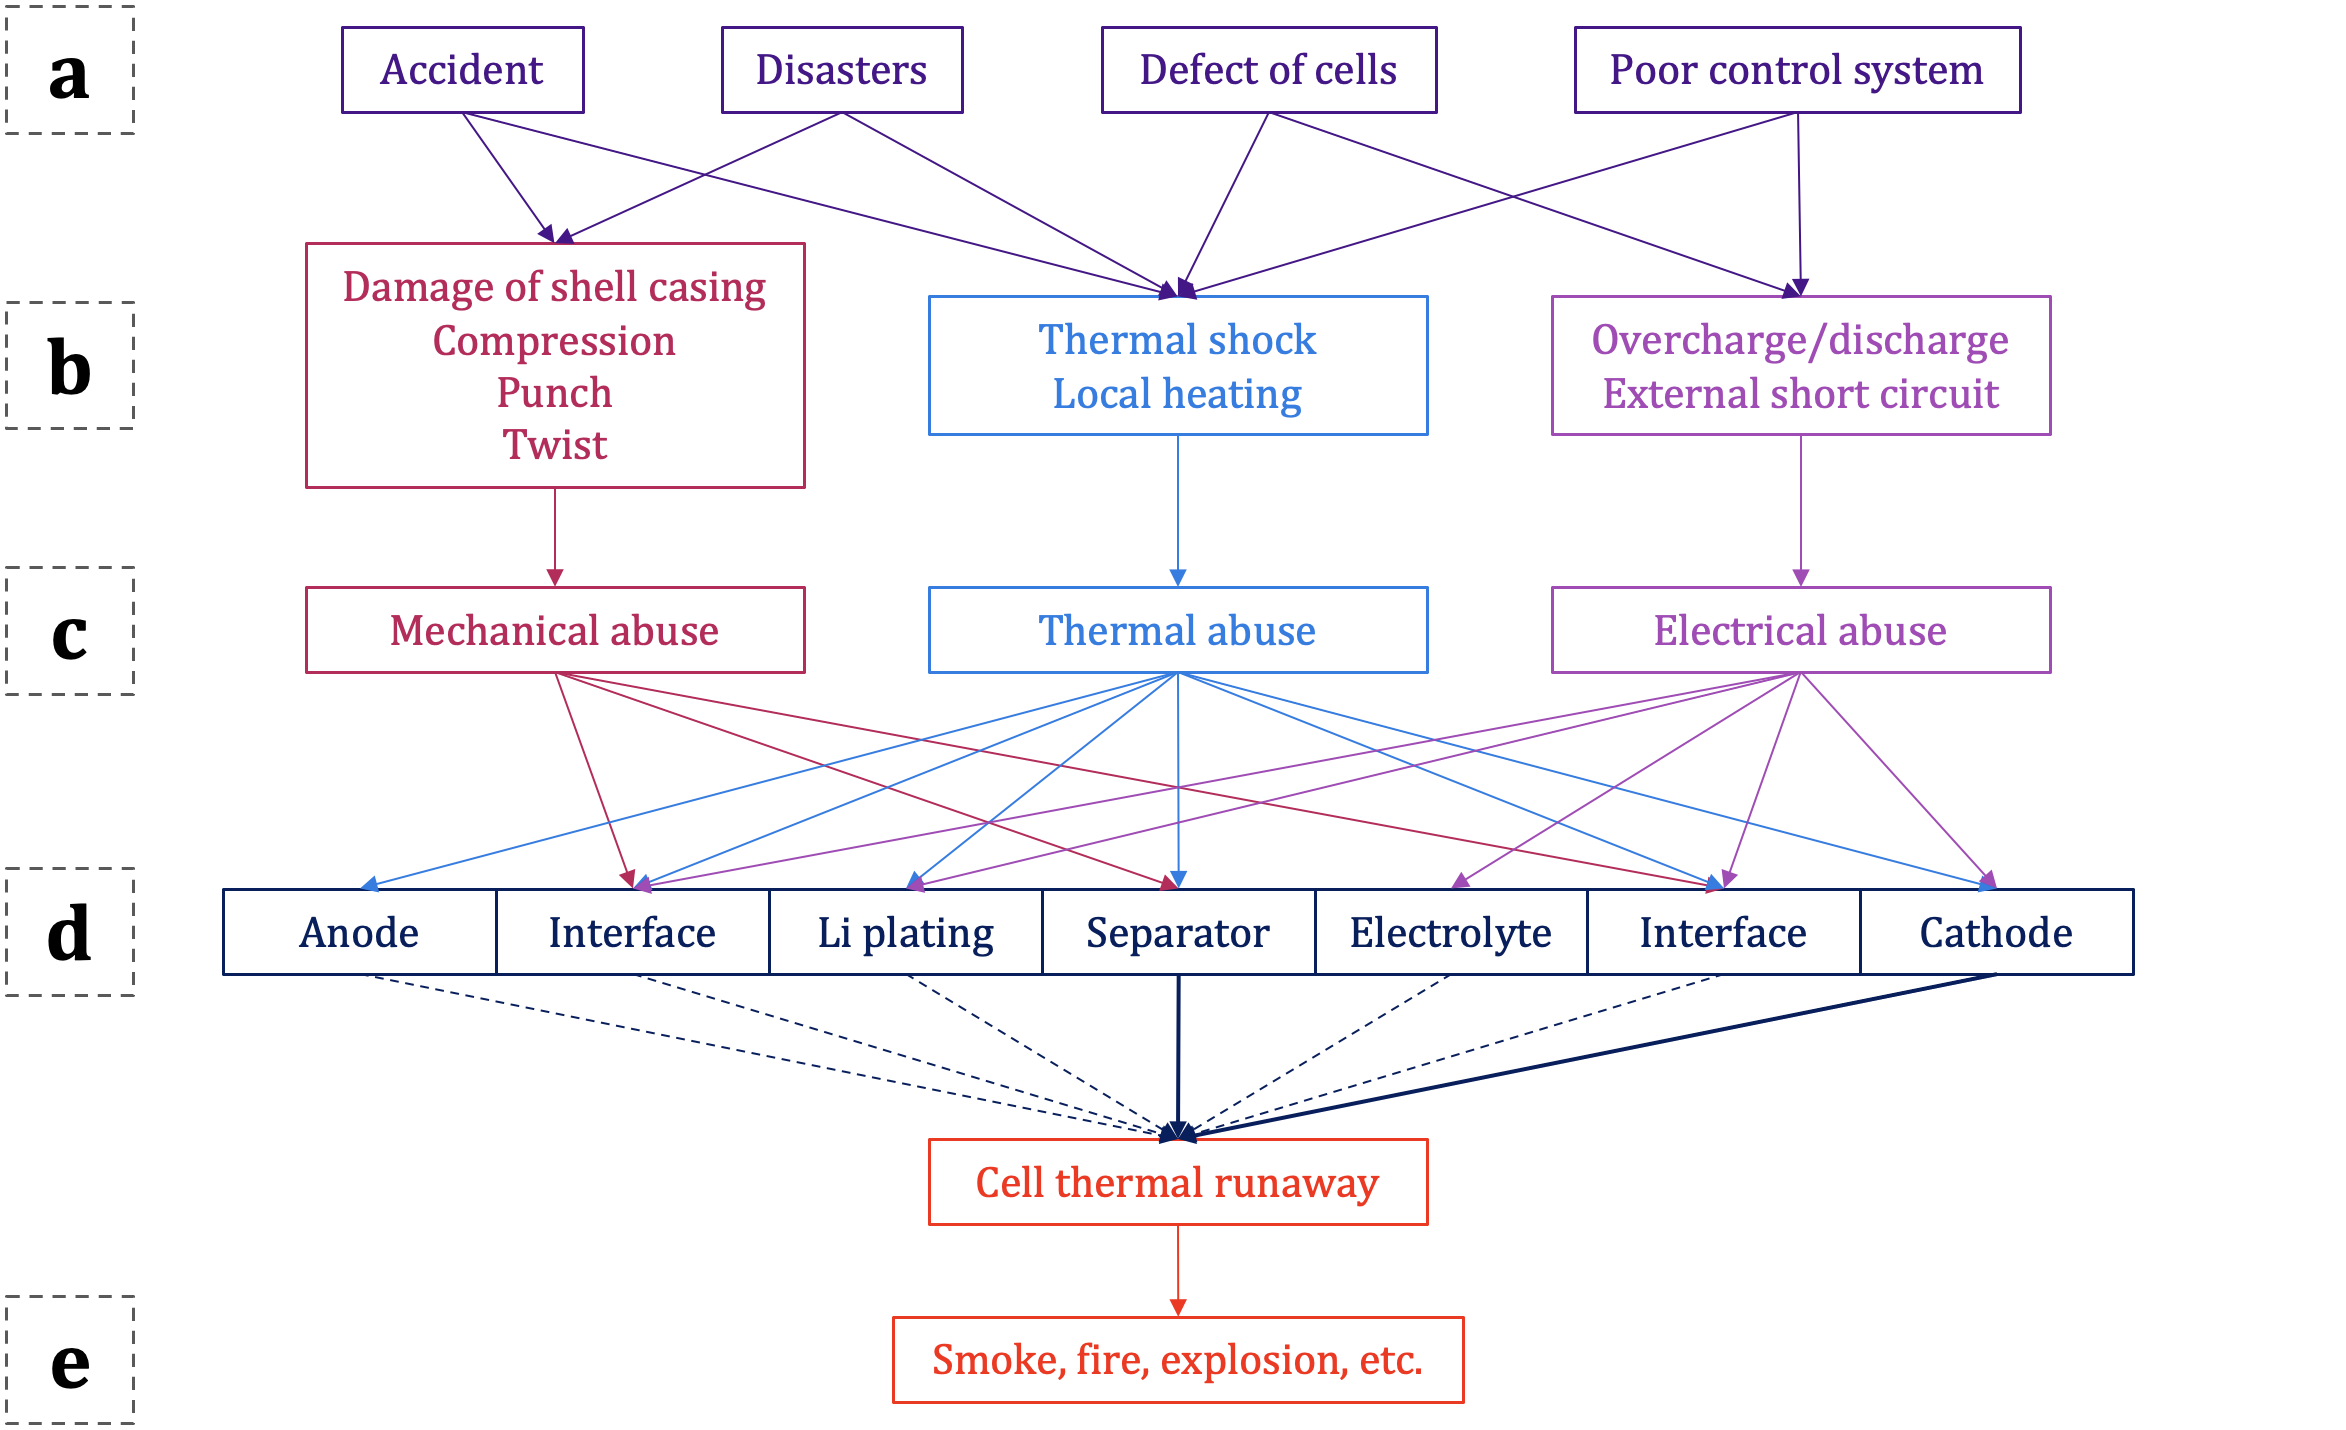
\includegraphics[width=0.9\textwidth]{Images/Chapter1/tr-graph.png}
    \caption[Schematic of the causes of lithium-ion battery thermal runaway]{Schematic of the causes of lithium-ion battery thermal runaway. Breakage of the separator and the oxygen evolution from the cathode side are the root causes to batteries' thermal runaway (as shown by the solid lines). Source: Chen (2020) \cite{chen2021review}.}
    \label{fig:tr-graph}
\end{figure}

\textbf{Queste frasi sono copiaincollate da} \texttt{chen2021review}\textbf{, quindi sono da riscrivere.}

Rising battery temperature would trigger other undesirable parasitic reactions, causing thermal runaway, where battery heat generation cannot be controlled \cite{wang2012thermal}.
During mechanical (damage to shell casing, compression, punching, and twisting of cells), electrical (overcharge/discharge and short circuit), and thermal abuse (thermal shock and local heating) situations, which could occur during accidents, thermal runaway will occur even quicker \cite{guo2010three,kim2007three,lamb2014evaluation}. Understanding LIB performance in unsafe conditions is critical, therefore, for the pro- duction of safer cells.

In the normal voltage and temperature range, only Li+ shuttle occurs in the electrolyte during the insertion/extraction cycles at the cathode and anode. At high-temperature and high-voltage conditions, the electrochemical reactions become more complex, including decomposition of the solid electrolyte interface (SEI) film, oxygen release at the cathode side, and additional electrolyte/electrode parasitic side reactions \cite{maleki1999thermal}. SEI film decomposition and interfacial reactions initially accelerate the temperature increase, thereby increasing risks of oxygen release from the active cathode materials. These reactions eventually lead to LIB thermal runaway, which causes battery rupture and explosion due to the reaction of hot flammable gases from the battery with the ambient oxygen \cite{finegan2016investigating}.

There are five types of causes for this phenomenon, which are illustrated in Fig. 2. The first type is uncontrollable internal heat generation, which causes oxygen release from the cathode material, leading to numerous side reactions [[37,53]]. In the second type, separator defects (due to thermally-induced shrinkage or mechan- ical damage) create short circuits in the battery and rapid discharge of the energy stored in it [[54]], accompanied by undesirable chemical chain reactions and release of massive amounts of heat. The third type is electrical abuse [[55]]. Electrolyte decomposition, especially in a high state of charge (SOC), occurs at the cathode interface. This leads to heat accumulation and consequently release of oxygen from the cathode and damage to the separator. The fourth type consists of electrochemical side reactions caused by local thermal abuse. If the heat generated during normal LIB operations cannot be dissipated quickly enough, the separator in that specific place will shrink or rupture [[41,56]]. The fifth type occurs during mechanical battery damage, which causes short circuits and/or air to penetrate the battery [[57]]. The main causes of battery safety accidents among these five categories are short-circuiting due to separator damage, electrical abuse, and mechanical abuse [[11,58]].

\textbf{Queste frasi sono copiaincollate da} \texttt{wang2012thermal}\textbf{, quindi sono da riscrivere.}

Generally, thermal runaway occurs when an exothermic reaction goes out of control, that is the reaction rate increases due to an increase in temperature causing a further increase in temperature and hence a further increase in the reaction rate [16,17], which possibly resulting in an explosion. It is proposed that above 80 $^\circ$C, thermal runaway can occur spontaneously as a result of fire or explosion [18]. For the lithium ion battery runaway, it is caused by the exothermic reactions between the electrolyte, anode and cathode, with the temperature and pressure increasing in the battery, the battery will rupture at last.

\begin{figure}[ht]
    \centering
    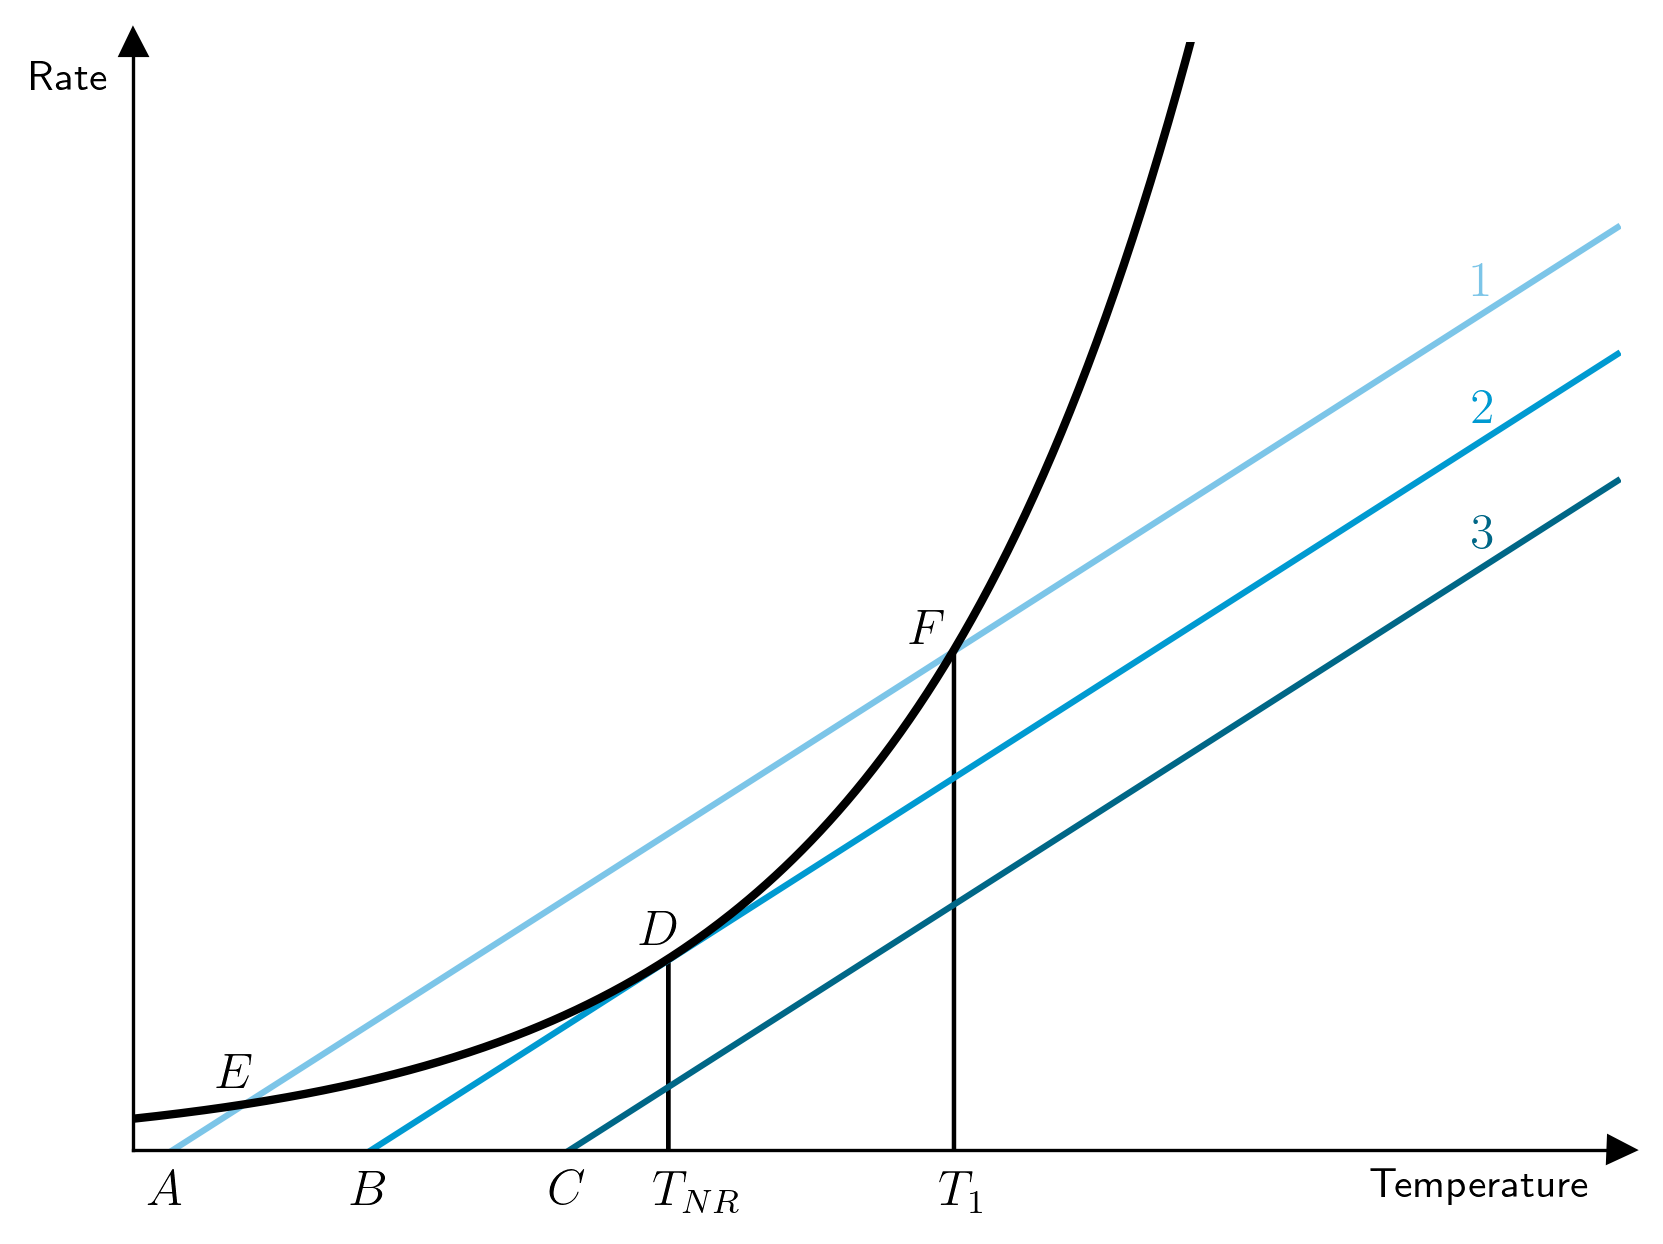
\includegraphics[width=0.7\textwidth]{Images/Chapter1/semenov-plot.png}
    \caption[Temperature dependence of reaction rate and heat loss]{Temperature dependence of reaction rate and heat loss from a system at three ambient temperature: $A$, $B$ and $C$. $A$ can control the sample temperature; $B$ is the critical temperature and the sample temperature can reach $T_{NR}$; if the ambient temperature exceeds $B$, the heat generation and losses are no longer balanced and the system will undergo thermal runaway. Source: Semenov (2013) \cite{semenov2013some}.}
    \label{fig:semenov-plot}
\end{figure}

Other info on thermal runaway can be found in "Thermal runaway - 2565" (in depth discussion), "Failure description - 43" (interesting perspective on the topic, it presents the failures per component with some nice graphs, in addition to in depth description of the reactions in thermal runaway), "Failure description - 890" (in depth discussion)

\section{Internal Short Circuit}
\label{sec:internal-short-circuit}

\section{Electric Failure and Abuse Testing}
\label{sec:electric-failure-abuse-testing}
Electric, Mechanical and Thermal failures can be found in "Safety Issues - 770"

\section{Mechanical Failure and Abuse Testing}
\label{sec:mechanical-failure-abuse-testing}

\section{Thermal Failure and Abuse Testing}
\label{sec:thermal-failure-abuse-testing}

\section{Safety Features in Commercial Batteries}
\label{sec:safety-features}
Can be found in "Safety Issues - 770", "Failure description - 43"

\section{CT for Degradation Studies}
\label{sec:ct-degradation-studies}

\chapter{Synchrotron X-Ray Imaging}
\label{ch:imaging}%
\section{X-ray Sources}
\label{sec:sources}

\subsection{European Synchrotron Radiation Facility (ESRF)}
\label{sec:esrf}

\subsubsection{Beamline ID19}
\label{sec:id19}

\section{Light-Matter Interaction}
\label{sec:light-matter}

\section{X-ray Computed Tomography}
\label{sec:xray-ct}

\chapter{CT-scans segmentation}
\label{ch:segmentation}%
\begin{algorithm}[H]
    \label{alg:segmentation}
    \caption{Segmentation algorithm}
    %\label{alg:var2}
    %\label{protocol2}
    \begin{algorithmic}[1]
    \STATE \textbf{SET} $hypervolume$, $hypervolume\_mask$
    \STATE $previous\_volume=hypervolume[0]$
    \STATE $threshold=\,$\texttt{find\_threshold}($previous\_volume$)
    \STATE $previous\_mask=\,$\texttt{segment3D}($previous\_volume$, $threshold$)
    \STATE \texttt{filtering3D}($previous\_mask$)
    \STATE \texttt{rename\_labels}($previous\_mask$)
    \STATE $hypervolume\_mask[0]=previous\_mask$s
    \FOR{$t=1$ to $end$}
    \STATE $current\_volume=hypervolume[t]$
    \STATE $current\_mask=\,$\texttt{segment3D}($current\_volume$, $threshold$)
    \STATE \texttt{filtering3D}($previous\_mask$)
    \STATE $current\_mask=\,$\texttt{propagate\_labels}($previous\_mask$, $current\_mask$)    
    \STATE \texttt{rename\_labels}($current\_mask$)
    \STATE $hypervolume\_mask[t]=current\_mask$
    \STATE $previous\_mask=current\_mask$
    \ENDFOR
    \end{algorithmic}
\end{algorithm}

\begin{algorithm}[H]
    \label{alg:segmentation2}
    \caption{Segmentation algorithm}
    %\label{alg:var2}
    %\label{protocol2}
    \begin{algorithmic}[1]
    \STATE get the hypervolume memmap and initialize the hypervolume mask memmap
    \STATE set previous volume to the first volume in the hypervolume
    \STATE find the threshold using previous volume
    \STATE segment the previous volume with the threshold and get previous mask
    \STATE filter previous mask
    \STATE rename the labels in previous mask
    \STATE set the first mask in the hypervolume mask to previous mask
    \FOR{$t=1$ to $end$}
    \STATE set current volume to the volume at time $t$ in the hypervolume
    \STATE segment current volume with the threshold and get current mask
    \STATE filter current mask
    \STATE propagate the labels from previous mask to current mask
    \STATE rename the labels in current mask
    \STATE set the mask at time $t$ in the hypervolume mask to current mask
    \STATE set previous mask to current mask
    \ENDFOR
    \end{algorithmic}
\end{algorithm}

% \chapter{Useful Things}
% \label{ch:usefulthings}%
% The \label{...}% enables to remove the small indentation that is generated, always leave the % symbol.

\chapter{Conclusions and future developments}
\label{ch:conclusions}%
A final chapter containing the main conclusions of your research/study and possible future developments of your work have to be inserted in this chapter.

%-------------------------------------------------------------------------
%	BIBLIOGRAPHY
%-------------------------------------------------------------------------

\addtocontents{toc}{\vspace{2em}} % Add a gap in the Contents, for aesthetics
\bibliography{Thesis_bibliography} % The references information are stored in the file named "Thesis_bibliography.bib"

%-------------------------------------------------------------------------
%	APPENDICES
%-------------------------------------------------------------------------

\cleardoublepage
\addtocontents{toc}{\vspace{2em}} % Add a gap in the Contents, for aesthetics
\appendix
\chapter{Appendix A}
\label{ch:appendixA}%
\input{Chapters/AppendixA.tex}


% LIST OF FIGURES
\listoffigures

% LIST OF TABLES
\listoftables

% LIST OF SYMBOLS
% Write out the List of Symbols in this page
% \chapter*{List of Symbols} % You have to include a chapter for your list of symbols (
% \begin{table}[H]
%     \centering
%     \begin{tabular}{lll}
%         \textbf{Variable} & \textbf{Description} & \textbf{SI unit} \\\hline\\[-9px]
%         $\bm{u}$ & solid displacement & m \\[2px]
%         $\bm{u}_f$ & fluid displacement & m \\[2px]
%     \end{tabular}
% \end{table}

% ACKNOWLEDGEMENTS
\chapter*{Acknowledgements}
Here you might want to acknowledge someone.

\cleardoublepage

\end{document}
